This chapter describes tasks which are generally not recommended to users new to Ubuntu since it involves risk and could lead to issues. The instructions below should be followed only if you are capable of solving problems which might rise and also preferably not your production computer.

%% Sections which are postponed to future editions of this manual. Currently present here as a reminder. Please do not delete!
%\section{Networking via Samba}
%\section{Remote Desktop}
%\section{Installing application from source}

\section{Installing other desktop shells (GNOME Shell, GNOME Classic)} \index{GNOME}
Although Unity is an excellent working environment, there are times when a user may wish to run an alternate desktop shell. Many such shells are available and run from minimalist, keyboard driven interfaces (e.g. DWM, Awesome, Xmonad, i3 etc.) to fully featured environments with dedicated applications (e.g. GNOME Shell, KDE, XFCE, LXDE etc.). \index{KDE} \index{XFCE} \index{LXDE} For the purposes of this example, consider a user who wishes to install GNOME Shell (the default graphical shell of the GNOME 3 project) as well as the GNOME Classic Session (a shell which more closely resembles the previous GNOME 2 interface). \\

\subsection*{Installing GNOME Shell}
GNOME Shell is a package like any other applications. It was already described in chapter \ref{chap:software_management} how to install a package using the Ubuntu Software Center. The exact procedure will be followed here. Please refer to that section if you are unable to follow the steps given here in this section. Launch the Ubuntu Software Center using the dash or the launcher. Search for ``GNOME shell",  and then click Install. This is shown in figure \ref{fig:GNOMEshell1}.

\begin{figure}[h!]	
	\centering
	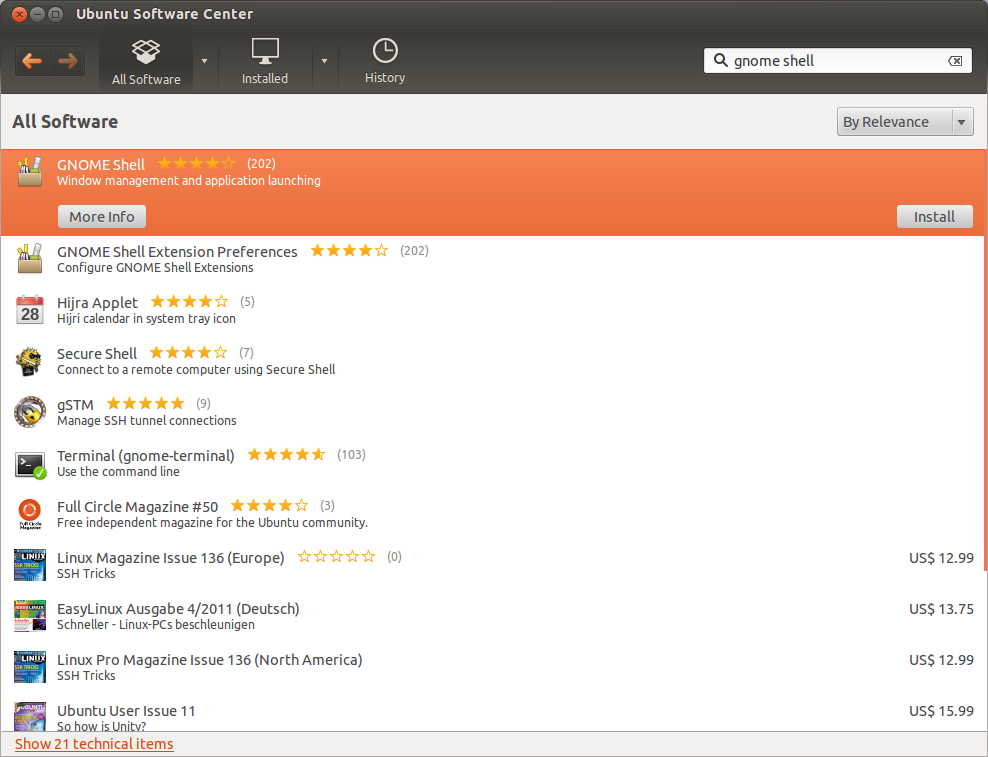
\includegraphics[width=350pt]{./images/advanced-topics/gnomeshell1.png}
	\caption{Install GNOME Shell using the Ubuntu Software Center}	
	\label{fig:GNOMEshell1}		
\end{figure}

\subsection*{GNOME Classic Session} \index{GNOME Classic}
In a similar fashion, to install the GNOME Classic Session, search for "gnome panel" in the Ubuntu Software Center and click Install. Alternatively, both desktop shells may be installed via the Terminal using the apt-get command. Since we are installing a package, we need to use the sudo command to install GNOME Shell or GNOME panel as an administrator. This is also shown here for reference in figure \ref{fig:GNOMEshell2}.

\begin{figure}[h!]	
	\centering
	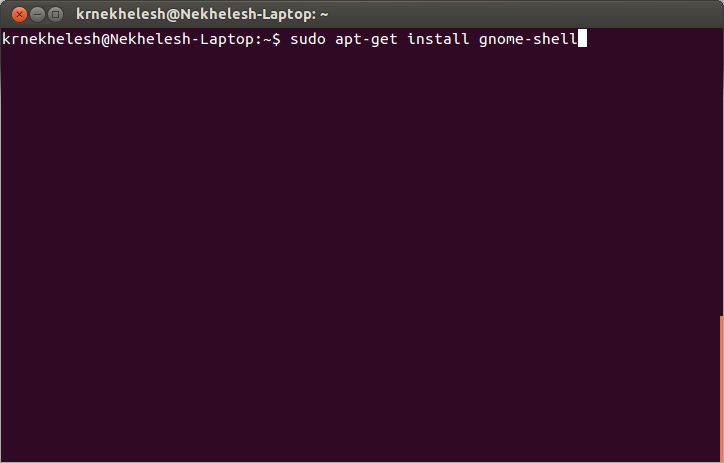
\includegraphics[width=300pt]{./images/advanced-topics/gnomeshell2.png}
	\caption{Install GNOME Shell using the terminal}	
	\label{fig:GNOMEshell2}		
\end{figure}

\par \noindent Once the installation is complete, simply log out of the Unity session, and click on the Ubuntu symbol to the right of the user name. A list of available desktop shells will appear, and a different session may be selected. This will return the user to the main login screen, and entering the password will launch the newly selected session (GNOME Shell, perhaps).